\documentclass[14pt]{extarticle}
\usepackage{fontspec}
\usepackage{polyglossia}
\usepackage{amsmath}
\usepackage{amssymb}
\usepackage{xcolor}
\usepackage{fancyhdr}
\usepackage{graphicx}
\usepackage{listings}
\usepackage[most]{tcolorbox}
% \usepackage{setspace}
\usepackage{pifont}
\usepackage{enumitem}
\usepackage{titlesec}
\usepackage[bottom]{footmisc}
\usepackage{titling}
\usepackage{minted}
\usepackage{etoolbox}
\usepackage{array}
\usepackage{extsizes}
\usepackage{float}
\usepackage{booktabs}
\usepackage{hyperref}
\usepackage[onehalfspacing]{setspace}
\usepackage[a4paper, top=2.7cm, bottom=2.7cm, left=2.5cm, right=2.5cm, headheight=1.5cm, headsep=0.5cm]{geometry}
\usepackage{tikz}

\usetikzlibrary{automata, positioning, arrows.meta, arrows}

\newfontfamily\emoji{Segoe UI Emoji}

\pagestyle{fancy}

\setmainlanguage[numerals=western]{arabic}
\setotherlanguage{english}
% \newfontfamily\arabicfont[Script=Arabic]{Amiri}
\newfontfamily\arabicfont[Script=Arabic]{Calibri}
\newfontfamily\arabicfonttt[Script=Arabic]{Courier New}

\lstset{
  language=[Sharp]C,
  numbers=left,
  stepnumber=1,
  numbersep=8pt,
  frame=single,
  basicstyle=\ttfamily\small,
  keywordstyle=\color{blue},
  stringstyle=\color{red},
  commentstyle=\color{green!50!black}
}

\newif\ifdetailed
\ifdefined\setdetailed
  \setdetailed
\fi

\newif\ifwithsols
\ifdefined\setwithsols
  \setwithsols
\fi

% unified tcolorboxes for articles
\tcbset{colback=white, colframe=black, fonttitle=\bfseries, boxrule=0.8pt}
\newtcolorbox{boxDef}[1][]{colback=blue!5!white,colframe=blue!75!black,
  title={{\emoji📘} تعريف\ifx\\#1\\\else ~#1\fi :}}
\newtcolorbox{boxExercise}[1][]{colback=cyan!5!white,colframe=cyan!70!black,
  title={{\emoji🧩} تمرين\ifx\\#1\\\else ~#1\fi :}}
\newtcolorbox{boxExample}[1][]{colback=yellow!5!white,colframe=orange!90!black,
  title={{\emoji📝} مثال\ifx\\#1\\\else ~#1\fi :}}
\newtcolorbox{boxNote}[1][]{colback=gray!10!white,colframe=black,
  title={{\emoji✨} ملاحظة\ifx\\#1\\\else ~#1\fi :}}
\newtcolorbox{boxAttention}[1][]{colback=magenta!10!white,colframe=magenta!80!black,
  title={{\emoji🔔} تنبيه\ifx\\#1\\\else ~#1\fi :}}
\newtcolorbox{boxWarning}[1][]{colback=red!5!white,colframe=red!75!black,
  title={{\emoji⚡} ملاحظة هامة\ifx\\#1\\\else ~#1\fi :}}
\newtcolorbox{boxSolution}[1][]{colback=green!5!white,colframe=green!60!black,
  title={{\emoji✅} حل\ifx\\#1\\\else ~#1\fi :}}
\newtcolorbox{boxSymbol}[1][]{colback=purple!5!white,colframe=purple!70!black,
  title={{\emoji🔣} رمز\ifx\\#1\\\else ~#1\fi :}}
\newtcolorbox{boxHint}[1][]{colback=teal!5!white,colframe=teal!60!black,
  title={{\emoji💡} تلميح\ifx\\#1\\\else ~#1\fi :}}


\tcbset{simplecode/.style={ colback=gray!5, colframe=black!50, boxrule=0.4pt, arc=2pt, left=4pt,right=4pt,top=4pt,bottom=4pt}}
\newenvironment{boxCode}{\begin{tcolorbox}[simplecode]}{\end{tcolorbox}}

\newcolumntype{C}[1]{>{\centering\arraybackslash}p{#1}}

% redefine spaces after titles
\makeatletter
\renewcommand{\@maketitle}{%
  \begin{center}
    {\huge \bfseries \@title \par}%
    \vskip 0.2em % space between title and author
    {\large \@author \par}%
    % \vskip 0.2em % space between author and date
    % {\normalsize \@date \par}%
  \end{center}
}
\makeatother

\fancyhf{} % clear default
\fancypagestyle{plain}{
  \fancyhf{}
  \fancyhead[L]{مدرسة التسامح الشاملة}
  % \fancyhead[L]{
\includegraphics[height=1cm]{../../../images/logoTasamoh.png}}
  \fancyhead[R]{الأستاذ محمود اغبارية}
  \fancyfoot[C]{\thepage}
}

\fancyhead[L]{مدرسة التسامح الشاملة}
\fancyhead[R]{الأستاذ محمود اغبارية}
\fancyfoot[C]{\thepage}
% \date{\today}

\setcounter{tocdepth}{3} % only section subsection and subsubsection in TOC

\newcommand{\importpdfpage}[2]{%
    \thispagestyle{empty}
    \newgeometry{left=0cm,right=0cm,top=0cm,bottom=0cm}
    \includegraphics[page=#2,width=0.95\paperwidth,height=0.95\paperheight,keepaspectratio]{#1}
    \restoregeometry
}

\newcommand{\insertFullImg}[1]{%
    \noindent
    \makebox[\textwidth][c]{
        \includegraphics[width=0.9\paperwidth,keepaspectratio]{#1}%
    }%
}%

% ----------------------


% \begin{document}

% \maketitle

% % \clearpage  % start TOC on a new page
% % \renewcommand{\contentsname}{جدول المحتويات}
% % \tableofcontents
% % \clearpage

% \part*{part 1} % the * prevents numbering
% \section*{مقدمة}
% \subsection*{مثال رياضي}
% \subsubsection*{مثال فرعي}
% \paragraph*{ paragraph 1}
% \subparagraph*{sub paragraph 1}

% \ifdetailed
% \begin{english}
% \begin{minted}{csharp}
% // C# Example
% \end{minted}
% \end{english}
% \fi

% OLD WAY
% \ifdetailed
% \begin{english}
% \begin{lstlisting}
% // C# Example
% \end{lstlisting}
% \end{english}
% \fi

% % 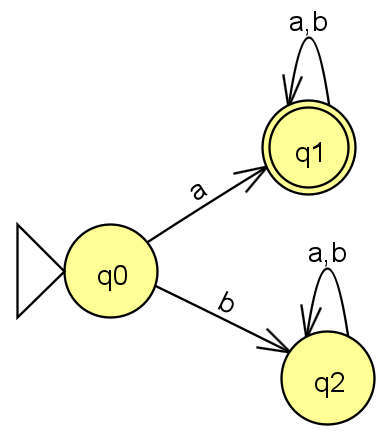
\includegraphics[width=0.2\textwidth]{../../../images/DFAs/ex1_q1.png}



% \vspace{3cm}
% \begin{flushleft}
% أرجو لكم وقتًا ممتعًا.

% الأستاذ محمود اغبارية.
% \end{flushleft}


% \end{document}


\ifwithsols
\title{حل تمرين 1 - آلة تيورينج}
\else
\title{تمرين 1 - آلة تيورينج}
\fi

\begin{document}

\maketitle

%%%%%%%%%%%%%%%%%%%%%%%%%%%%%%%%%%%%%%%%%%
\section{تحليل الآلة}
%%%%%%%%%%%%%%%%%%%%%%%%%%%%%%%%%%%%%%%%%%

لكل آلة من الآلات التالية، حدد اللغة التي تقبلها، وأعطِ مثالاً على كلمة مقبولة وكلمة مرفوضة.

\ifwithsols
\begin{enumerate}[itemsep=4em]
\else
\begin{enumerate}[itemsep=2em]
\fi

%--- Q1 ---
\item
\begin{center}
\begin{tikzpicture}[->,>=stealth',shorten >=1pt,auto,node distance=3.2cm,thick]
    \node[state,initial] (q0) {$q_0$};
    \node[state,accepting] (q1) [right of=q0] {$q_1$};

    \path (q0) edge[loop above] node {$a \mid a, R$} (q0)
          (q0) edge node {$\triangle \mid \triangle, R$} (q1);
\end{tikzpicture}
\end{center}

\ifwithsols
\begin{boxSolution}
اللغة هي كل الكلمات المكونة من أحرف $a$ فقط، بما فيها الكلمة الفارغة:
\[ L = \{ a^n \mid n \geq 0 \} = a^* \]
\begin{itemize}
    \item كلمة مقبولة: $aaa$
    \item كلمة مرفوضة: $ab$ (الآلة تتوقف في $q_0$ عند قراءة $b$، وهي ليست حالة قابلة)
\end{itemize}
\end{boxSolution}
\clearpage
\fi

%--- Q2 ---
\item
\begin{center}
\begin{tikzpicture}[->,>=stealth',shorten >=1pt,auto,node distance=3.2cm,thick]
    \node[state,initial] (q0) {$q_0$};
    \node[state] (q1) [right of=q0] {$q_1$};
    \node[state,accepting] (q2) [right of=q1] {$q_2$};

    \path (q0) edge node {$a \mid X, R$} (q1)
          (q1) edge[loop above] node {$a \mid a, R$} (q1)
          (q1) edge node {$b \mid X, R$} (q2)
          (q2) edge[loop above] node {$b \mid b, R$} (q2);
\end{tikzpicture}
\end{center}

\ifwithsols
\begin{boxSolution}
تبحث الآلة عن أول $a$ تشطبها، ثم تمر على بقية الـ $a$، ثم تبحث عن أول $b$ تشطبها وتصل إلى الحالة القابلة.\\
\textbf{ملاحظة:} الحالة $q_2$ قابلة وفيها حلقة على $b$، لذلك يمكن أن تبقى فيها.\\
اللغة هي كل الكلمات من الشكل $a^m b^n$ حيث $m, n \geq 1$:
\[ L = \{ a^m b^n \mid m, n \geq 1 \} \]
\begin{itemize}
    \item كلمة مقبولة: $aabb$
    \item كلمة مرفوضة: $ba$ (تتوقف في $q_0$ لأنه لا يوجد انتقال على $b$)
\end{itemize}
\end{boxSolution}
\fi

%--- Q3 ---
\item
\begin{center}
\begin{tikzpicture}[->,>=stealth',shorten >=1pt,auto,node distance=3cm,thick]
    \node[state,initial] (q0) {$q_0$};
    \node[state] (q1) [right of=q0] {$q_1$};
    \node[state] (q2) [right of=q1] {$q_2$};
    \node[state,accepting] (q3) [right of=q2] {$q_3$};

    \path (q0) edge node {$a \mid X, R$} (q1)
          (q1) edge[loop above] node {$a \mid a, R$} (q1)
          (q1) edge node {$b \mid Y, R$} (q2)
          (q2) edge[loop above] node {$b \mid b, R$} (q2)
          (q2) edge node {$c \mid Z, R$} (q3)
          (q3) edge[loop above] node {$c \mid c, R$} (q3);
\end{tikzpicture}
\end{center}

\ifwithsols
\begin{boxSolution}
تشطب الآلة أول $a$ ثم أول $b$ ثم أول $c$ وتصل إلى الحالة القابلة، وتبقى فيها مع بقية الـ $c$.\\
اللغة هي كل الكلمات من الشكل $a^m b^n c^k$ حيث $m, n, k \geq 1$:
\[ L = \{ a^m b^n c^k \mid m, n, k \geq 1 \} \]
\begin{itemize}
    \item كلمة مقبولة: $abcc$
    \item كلمة مرفوضة: $ac$ (لا يوجد انتقال من $q_1$ على $c$)
\end{itemize}
\end{boxSolution}
\clearpage
\fi

\end{enumerate}

%%%%%%%%%%%%%%%%%%%%%%%%%%%%%%%%%%%%%%%%%%
\clearpage
\section{تتبع تنفيذ الآلة}
%%%%%%%%%%%%%%%%%%%%%%%%%%%%%%%%%%%%%%%%%%

\ifwithsols
\begin{enumerate}[itemsep=4em]
\else
\begin{enumerate}[itemsep=2em]
\fi

%--- Q4 ---
\item
فيما يلي آلة تيورينج:

\begin{center}
\begin{tikzpicture}[->,>=stealth',shorten >=1pt,auto,node distance=3cm,thick]
    \node[state,initial] (q0) {$q_0$};
    \node[state] (q1) [right of=q0] {$q_1$};
    \node[state] (q2) [right of=q1] {$q_2$};
    \node[state,accepting] (q3) [below of=q1] {$q_3$};

    \path (q0) edge node {$a \mid X, R$} (q1)
          (q1) edge[loop above] node {$a \mid a, R$} (q1)
          (q1) edge node {$b \mid Y, L$} (q2)
          (q2) edge[loop above] node {$a \mid a, L$} (q2)
          (q2) edge node[left] {$X \mid X, R$} (q0)
          (q0) edge node[right] {$Y \mid Y, R$} (q3)
          (q3) edge[loop below] node {$Y \mid Y, R$} (q3);
\end{tikzpicture}
\end{center}

\begin{enumerate}
    \item تتبّع تنفيذ الآلة على الكلمة $w = aab$. ما هو مضمون الشريط عند التوقف؟
    \item تتبّع تنفيذ الآلة على الكلمة $w = ab$. ما هو مضمون الشريط عند التوقف؟
    \item تتبّع تنفيذ الآلة على الكلمة $w = aabb$. هل تُقبل؟
    \item ما اللغة التي تقبلها هذه الآلة؟
\end{enumerate}

\ifwithsols
\begin{boxSolution}

\textbf{أ. تتبع على $w = aab$:}
\begin{align*}
q_0 \quad &\vdash \, \underline{a} \, a \, b \, \triangle \, \ldots \\
q_1 \quad &\vdash \, X \, \underline{a} \, b \, \triangle \, \ldots \\
q_1 \quad &\vdash \, X \, a \, \underline{b} \, \triangle \, \ldots \\
q_2 \quad &\vdash \, X \, \underline{a} \, Y \, \triangle \, \ldots \\
q_2 \quad &\vdash \, \underline{X} \, a \, Y \, \triangle \, \ldots \\
q_0 \quad &\vdash \, X \, \underline{a} \, Y \, \triangle \, \ldots \\
q_1 \quad &\vdash \, X \, X \, \underline{Y} \, \triangle \, \ldots \\
\end{align*}
لا يوجد انتقال من $q_1$ على $Y$، تتوقف الآلة. الكلمة مرفوضة.

\textbf{ب. تتبع على $w = ab$:}
\begin{align*}
q_0 \quad &\vdash \, \underline{a} \, b \, \triangle \, \ldots \\
q_1 \quad &\vdash \, X \, \underline{b} \, \triangle \, \ldots \\
q_2 \quad &\vdash \, \underline{X} \, Y \, \triangle \, \ldots \\
q_0 \quad &\vdash \, X \, \underline{Y} \, \triangle \, \ldots \\
q_3 \quad &\vdash \, X \, Y \, \underline{\triangle} \, \ldots \quad \checkmark
\end{align*}
الكلمة مقبولة. الشريط: $\vdash \, X \, Y \, \triangle \, \ldots$

\textbf{ج. تتبع على $w = aabb$:}
الآلة تشطب $a$ أولى وتبحث عن أول $b$. بعد شطب أول $b$ ترجع إلى بداية الشريط. تشطب $a$ ثانية وتبحث عن $b$ لكنها تجد $Y$، فتتوقف في $q_1$. الكلمة \textbf{مرفوضة}.

\textbf{د.} تقبل الآلة اللغة: $L = \{ a^n b^n \mid n \geq 1 \}$

في كل دورة تشطب $a$ واحدة و $b$ واحدة. إذا انتهت الأحرف معًا تنتقل إلى $q_3$.
\end{boxSolution}
\clearpage
\fi

\end{enumerate}

%%%%%%%%%%%%%%%%%%%%%%%%%%%%%%%%%%%%%%%%%%
\clearpage
\section{إكمال الآلة الناقصة}
%%%%%%%%%%%%%%%%%%%%%%%%%%%%%%%%%%%%%%%%%%

أكمل الانتقالات الناقصة في كل آلة من الآلات التالية.

\ifwithsols
\begin{enumerate}[itemsep=4em]
\else
\begin{enumerate}[itemsep=3em]
\fi

%--- Q5 ---
\item
الآلة تقبل اللغة $L = \{a^n b^n \mid n \geq 0\}$ (بما فيها الكلمة الفارغة).\\
أكمل الانتقالات الناقصة (المشار إليها بـ ؟):

\begin{center}
\begin{tikzpicture}[->,>=stealth',shorten >=1pt,auto,node distance=3cm,thick]
    \node[state,initial] (q0) {$q_0$};
    \node[state] (q1) [right of=q0] {$q_1$};
    \node[state] (q2) [right of=q1] {$q_2$};
    \node[state] (q3) [below of=q0] {$q_3$};
    \node[state,accepting] (q4) [right of=q3] {$q_4$};

    \path (q0) edge node {$a \mid X, R$} (q1)
          (q0) edge node[left] {$? \mid ?, ?$} (q3)
          (q1) edge[loop above] node {$a \mid a, R$} (q1)
          (q1) edge[loop below] node {$Y \mid Y, R$} (q1)
          (q1) edge node {$b \mid Y, L$} (q2)
          (q2) edge[loop above] node {$? \mid ?, ?$} (q2)
          (q2) edge[loop right] node {$? \mid ?, ?$} (q2)
          (q2) edge node[right] {$X \mid X, R$} (q0)
          (q3) edge[loop below] node {$? \mid ?, ?$} (q3)
          (q3) edge node {$\triangle \mid \triangle, R$} (q4);
\end{tikzpicture}
\end{center}

\ifwithsols
\begin{boxSolution}
\begin{center}
\begin{tikzpicture}[->,>=stealth',shorten >=1pt,auto,node distance=3cm,thick]
    \node[state,initial] (q0) {$q_0$};
    \node[state] (q1) [right of=q0] {$q_1$};
    \node[state] (q2) [right of=q1] {$q_2$};
    \node[state] (q3) [below of=q0] {$q_3$};
    \node[state,accepting] (q4) [right of=q3] {$q_4$};

    \path (q0) edge node {$a \mid X, R$} (q1)
          (q0) edge node[left] {\textcolor{red}{$Y \mid Y, R$}} (q3)
          (q1) edge[loop above] node {$a \mid a, R$} (q1)
          (q1) edge[loop below] node {$Y \mid Y, R$} (q1)
          (q1) edge node {$b \mid Y, L$} (q2)
          (q2) edge[loop above] node {\textcolor{red}{$a \mid a, L$}} (q2)
          (q2) edge[loop right] node {\textcolor{red}{$Y \mid Y, L$}} (q2)
          (q2) edge node[right] {$X \mid X, R$} (q0)
          (q3) edge[loop below] node {\textcolor{red}{$Y \mid Y, R$}} (q3)
          (q3) edge node {$\triangle \mid \triangle, R$} (q4);
\end{tikzpicture}
\end{center}

\textbf{شرح الانتقالات المكملة (باللون الأحمر):}
\begin{itemize}
    \item $q_0 \xrightarrow{Y \mid Y, R} q_3$: بعد انتهاء جميع الـ $a$، الموجود هو $Y$، ننتقل للتحقق من النهاية
    \item حلقة $q_2$ على $a \mid a, L$: عند العودة، نتجاوز الـ $a$ غير المشطوبة
    \item حلقة $q_2$ على $Y \mid Y, L$: عند العودة، نتجاوز الـ $Y$ (الـ $b$ المشطوبة)
    \item حلقة $q_3$ على $Y \mid Y, R$: نمر على الأحرف المشطوبة حتى نصل إلى النهاية
\end{itemize}
\end{boxSolution}
\clearpage
\fi

%--- Q6 ---
\item
الآلة تقبل اللغة $L = \{ww^R \mid w \in \{a, b\}^*\}$ (الكلمات المتناظرة ذات الطول الزوجي).\\
أكمل الانتقالات الناقصة:

\begin{center}
\begin{tikzpicture}[->,>=stealth',shorten >=1pt,auto,node distance=3cm,thick]
    \node[state,initial] (q0) {$q_0$};
    \node[state] (q1) [above right of=q0, yshift=0.3cm] {$q_1$};
    \node[state] (q2) [below right of=q0, yshift=-0.3cm] {$q_2$};
    \node[state] (q3) [right of=q1, xshift=0.5cm] {$q_3$};
    \node[state] (q4) [right of=q2, xshift=0.5cm] {$q_4$};
    \node[state,accepting] (q5) [below of=q0, yshift=-1.5cm] {$q_5$};

    \path (q0) edge node[above left] {$a \mid X, R$} (q1)
          (q0) edge node[below left] {$b \mid X, R$} (q2)
          (q0) edge node[left] {$\triangle \mid \triangle, R$} (q5)
          (q1) edge[loop above] node {$a \mid a, R$} (q1)
          (q1) edge[loop right] node {$? \mid ?, ?$} (q1)
          (q1) edge node {$a \mid X, L$} (q3)
          (q2) edge[loop below] node {$? \mid ?, ?$} (q2)
          (q2) edge[loop right] node {$b \mid b, R$} (q2)
          (q2) edge node {$b \mid X, L$} (q4)
          (q3) edge[loop above] node {$? \mid ?, ?$} (q3)
          (q3) edge[bend right=20] node[above] {$X \mid X, R$} (q0)
          (q4) edge[loop below] node {$? \mid ?, ?$} (q4)
          (q4) edge[bend left=20] node[below] {$X \mid X, R$} (q0);
\end{tikzpicture}
\end{center}

\ifwithsols
\begin{boxSolution}
\begin{center}
\begin{tikzpicture}[->,>=stealth',shorten >=1pt,auto,node distance=3cm,thick]
    \node[state,initial] (q0) {$q_0$};
    \node[state] (q1) [above right of=q0, yshift=0.3cm] {$q_1$};
    \node[state] (q2) [below right of=q0, yshift=-0.3cm] {$q_2$};
    \node[state] (q3) [right of=q1, xshift=0.5cm] {$q_3$};
    \node[state] (q4) [right of=q2, xshift=0.5cm] {$q_4$};
    \node[state,accepting] (q5) [below of=q0, yshift=-1.5cm] {$q_5$};

    \path (q0) edge node[above left] {$a \mid X, R$} (q1)
          (q0) edge node[below left] {$b \mid X, R$} (q2)
          (q0) edge node[left] {$\triangle \mid \triangle, R$} (q5)
          (q1) edge[loop above] node {$a \mid a, R$} (q1)
          (q1) edge[loop right] node {\textcolor{red}{$b \mid b, R$}} (q1)
          (q1) edge node {$a \mid X, L$} (q3)
          (q2) edge[loop below] node {\textcolor{red}{$a \mid a, R$}} (q2)
          (q2) edge[loop right] node {$b \mid b, R$} (q2)
          (q2) edge node {$b \mid X, L$} (q4)
          (q3) edge[loop above] node {\textcolor{red}{$a \mid a, L$ \quad $b \mid b, L$}} (q3)
          (q3) edge[bend right=20] node[above] {$X \mid X, R$} (q0)
          (q4) edge[loop below] node {\textcolor{red}{$a \mid a, L$ \quad $b \mid b, L$}} (q4)
          (q4) edge[bend left=20] node[below] {$X \mid X, R$} (q0);
\end{tikzpicture}
\end{center}

\textbf{شرح الاستراتيجية:}
\begin{itemize}
    \item $q_0$: نقرأ الحرف الأول ونشطبه
    \begin{itemize}
        \item إذا $a$: نذهب إلى $q_1$ (نبحث عن $a$ في نهاية الكلمة)
        \item إذا $b$: نذهب إلى $q_2$ (نبحث عن $b$ في نهاية الكلمة)
    \end{itemize}
    \item $q_1$, $q_2$: نمر على جميع الأحرف (من الاثنين) حتى نصل إلى آخر حرف غير مشطوب
    \item $q_3$, $q_4$: نشطب الحرف الأخير المطابق ونرجع إلى $q_0$
    \item قبول الكلمة الفارغة: انتقال مباشر من $q_0$ على $\triangle$
\end{itemize}
\end{boxSolution}
\clearpage
\fi

\end{enumerate}

%%%%%%%%%%%%%%%%%%%%%%%%%%%%%%%%%%%%%%%%%%
\clearpage
\section{بناء الآلة}
%%%%%%%%%%%%%%%%%%%%%%%%%%%%%%%%%%%%%%%%%%

لكل لغة من اللغات التالية، صمم آلة تيورينج تقبلها، مع تتبع مثال على كلمة مقبولة.

\ifwithsols
\begin{enumerate}[itemsep=4em]
\else
\begin{enumerate}[itemsep=2em]
\fi

%--- Q7 ---
\item \textbf{اللغة:}
\[ L = \{a^n b^m \mid n, m \geq 1 \text{ و } n \leq m\} \]
أي الكلمات التي عدد الـ $a$ أقل من أو يساوي عدد الـ $b$.

\textbf{مثال:} $ab$, $abb$, $aaabbb$, $aaabbbbb \in L$ \quad و \quad $aab$, $aaabb \notin L$.

\ifwithsols
\begin{boxSolution}
\textbf{الاستراتيجية:}
\begin{enumerate}
    \item نشطب أول $a$ ونبحث عن أول $b$، نشطبها
    \item نرجع ونشطب $a$ ثانية، ثم $b$ ثانية، وهكذا
    \item إذا انتهت الـ $a$ قبل الـ $b$ أو في نفس الوقت، نقبل
    \item إذا انتهت الـ $b$ قبل الـ $a$، نرفض
\end{enumerate}

\begin{center}
\begin{tikzpicture}[->,>=stealth',shorten >=1pt,auto,node distance=3cm,thick]
    \node[state,initial] (q0) {$q_0$};
    \node[state] (q1) [right of=q0] {$q_1$};
    \node[state] (q2) [right of=q1] {$q_2$};
    \node[state] (q3) [below of=q2] {$q_3$};
    \node[state,accepting] (q4) [below of=q1] {$q_4$};

    \path (q0) edge node {$a \mid X, R$} (q1)
          (q0) edge node[left] {$Y \mid Y, R$} (q4)
          (q1) edge[loop above] node {$a \mid a, R$} (q1)
          (q1) edge[loop below] node {$Y \mid Y, R$} (q1)
          (q1) edge node {$b \mid Y, L$} (q2)
          (q2) edge[loop above] node {$a \mid a, L$ \quad $Y \mid Y, L$} (q2)
          (q2) edge node[right] {$X \mid X, R$} (q0)
          (q4) edge[loop left] node {$Y \mid Y, R$} (q4)
          (q4) edge[loop below] node {$b \mid b, R$} (q4);
\end{tikzpicture}
\end{center}

\textbf{تتبع على $w = abb$:}
\begin{align*}
q_0 \quad &\vdash \, \underline{a} \, b \, b \, \triangle \, \ldots \\
q_1 \quad &\vdash \, X \, \underline{b} \, b \, \triangle \, \ldots \\
q_2 \quad &\vdash \, \underline{X} \, Y \, b \, \triangle \, \ldots \\
q_0 \quad &\vdash \, X \, \underline{Y} \, b \, \triangle \, \ldots \\
q_4 \quad &\vdash \, X \, Y \, \underline{b} \, \triangle \, \ldots \\
q_4 \quad &\vdash \, X \, Y \, b \, \underline{\triangle} \, \ldots \quad \checkmark \text{ (مقبولة)}
\end{align*}
\end{boxSolution}
\clearpage
\fi

%--- Q8 ---
\item \textbf{اللغة:}
\[ L = \{ a^n b^n c^m \mid n \geq 1,\ m \geq 0 \} \]
أي الكلمات التي عدد الـ $a$ يساوي عدد الـ $b$، يليها أي عدد من الـ $c$ (بما فيه الصفر).

\textbf{مثال:} $ab$, $aabb$, $abcc$, $aabbccc \in L$ \quad و \quad $abc$, $aab \notin L$.

\ifwithsols
\begin{boxSolution}
\textbf{الاستراتيجية:}
\begin{enumerate}
    \item نشطب $a$ و $b$ في كل دورة (كما في مثال $a^n b^n$ في الشرح)
    \item بعد انتهاء جميع الـ $a$ و $b$، نسمح بأي عدد من الـ $c$
\end{enumerate}

\begin{center}
\begin{tikzpicture}[->,>=stealth',shorten >=1pt,auto,node distance=3cm,thick]
    \node[state,initial] (q0) {$q_0$};
    \node[state] (q1) [right of=q0] {$q_1$};
    \node[state] (q2) [right of=q1] {$q_2$};
    \node[state] (q3) [below of=q0] {$q_3$};
    \node[state] (q5) [below of=q1] {$q_5$};
    \node[state,accepting] (q4) [below of=q2] {$q_4$};

    \path (q0) edge node {$a \mid X, R$} (q1)
          (q0) edge node[left] {$Y \mid Y, R$} (q3)
          (q1) edge[loop above] node {$a \mid a, R$ \quad $Y \mid Y, R$} (q1)
          (q1) edge node {$b \mid Y, L$} (q2)
          (q2) edge[loop above] node {$a \mid a, L$ \quad $Y \mid Y, L$} (q2)
          (q2) edge node[right] {$X \mid X, R$} (q0)
          (q3) edge[loop left] node {$Y \mid Y, R$} (q3)
          (q3) edge node {$\triangle \mid \triangle, R$} (q4)
          (q3) edge node {$c \mid c, R$} (q5)
          (q5) edge[loop right] node {$c \mid c, R$} (q5)
          (q5) edge node {$\triangle \mid \triangle, R$} (q4);
\end{tikzpicture}
\end{center}

\textbf{تتبع على $w = aabbcc$:}
\begin{align*}
q_0 \quad &\vdash \, \underline{a} \, a \, b \, b \, c \, c \, \triangle \\
&\ldots\text{(دورتان من الشطب)}\\
q_3 \quad &\vdash \, X \, X \, Y \, Y \, \underline{c} \, c \, \triangle \\
q_5 \quad &\vdash \, X \, X \, Y \, Y \, c \, \underline{c} \, \triangle \\
q_5 \quad &\vdash \, X \, X \, Y \, Y \, c \, c \, \underline{\triangle} \\
q_4 \quad &\ldots \quad \checkmark
\end{align*}
\end{boxSolution}
\clearpage
\fi

%--- Q9 ---
\item \textbf{اللغة:}
\[ L = \{ a^n b^m \mid n, m \geq 0 \text{ و } n \neq m \} \]
أي الكلمات التي عدد الـ $a$ يختلف عن عدد الـ $b$.

\textbf{مثال:} $a$, $bb$, $aaab$, $abbb \in L$ \quad و \quad $\varepsilon$, $ab$, $aabb \notin L$.

\textbf{تلميح:} اقسم الحل إلى حالتين - متى يكون $n > m$؟ ومتى يكون $n < m$؟

\ifwithsols
\begin{boxSolution}
\textbf{الاستراتيجية:}
نبني مساراً لكل حالة:
\begin{itemize}
    \item \textbf{المسار 1} ($n > m$): نشطب $a$ و $b$ بالتساوي. إذا انتهت الـ $b$ وبقيت $a$، نقبل.
    \item \textbf{المسار 2} ($n < m$): نشطب $a$ و $b$ بالتساوي. إذا انتهت الـ $a$ وبقيت $b$، نقبل.
\end{itemize}

\begin{center}
\begin{tikzpicture}[->,>=stealth',shorten >=1pt,auto,node distance=2.8cm,thick, scale=0.9, every node/.style={scale=0.9}]
    % Path 1: n > m
    \node[state,initial] (q0) {$q_0$};
    \node[state] (q1) [right of=q0] {$q_1$};
    \node[state] (q2) [right of=q1] {$q_2$};
    \node[state] (q3) [below of=q2] {$q_3$};
    \node[state,accepting] (qA) [below of=q1] {$q_A$};
    % Path 2: n < m
    \node[state] (q4) [below of=q0] {$q_4$};
    \node[state] (q5) [below of=q4] {$q_5$};
    \node[state,accepting] (qB) [right of=q5] {$q_B$};

    % Path 1 transitions
    \path (q0) edge node {$a \mid X, R$} (q1)
          (q1) edge[loop above] node {$a \mid a, R$ \quad $Y \mid Y, R$} (q1)
          (q1) edge node {$b \mid Y, L$} (q2)
          (q2) edge[loop above] node {$a \mid a, L$ \quad $Y \mid Y, L$} (q2)
          (q2) edge node[right] {$X \mid X, R$} (q0)
          (q0) edge node[left] {$Y \mid Y, R$} (q3)
          (q3) edge[loop right] node {$Y \mid Y, R$} (q3)
          (q3) edge[bend right] node {$a \mid a, R$} (qA)
          (qA) edge[loop below] node {$a \mid a, R$} (qA)
          % Path 2
          (q0) edge node[left] {$b \mid b, R$} (q4)
          (q4) edge[loop left] node {$b \mid b, R$} (q4)
          (q4) edge node[left] {$\triangle \mid \triangle, R$} (q5)
          (q5) edge node {$b \mid b, R$} (qB)
          (qB) edge[loop below] node {$b \mid b, R$} (qB);
\end{tikzpicture}
\end{center}

\textbf{ملاحظة:} المسار 2 يُفعَّل فقط عندما تبدأ الكلمة بـ $b$ (أي $n=0$ و $m>0$). \\
للحالة العامة $n < m$ (حيث $n > 0$)، يُكمل المسار 1 مرحلة الشطب حتى تنتهي الـ $a$، ثم تنتقل عبر $q_3$ ويجد $b$ متبقية فيقبل.
\end{boxSolution}
\clearpage
\fi

%--- Q10 ---
\item \textbf{اللغة:}
\[ L = \{ a^{2n} \mid n \geq 1 \} \]
أي الكلمات التي تتكون فقط من عدد \textbf{زوجي} من الأحرف $a$، وهذا العدد أكبر من الصفر.

\textbf{مثال:} $aa$, $aaaa$, $aaaaaa \in L$ \quad و \quad $\varepsilon$, $a$, $aaa \notin L$.

\textbf{تلميح:} فكر في كيفية التحقق من أن عدد الأحرف زوجي باستخدام الحالات فقط.

\ifwithsols
\begin{boxSolution}
\textbf{الفكرة:} نمر على الأحرف نأخذ اثنتين في كل مرة.

\begin{center}
\begin{tikzpicture}[->,>=stealth',shorten >=1pt,auto,node distance=3cm,thick]
    \node[state,initial] (q0) {$q_0$};
    \node[state] (q1) [right of=q0] {$q_1$};
    \node[state] (q2) [right of=q1] {$q_2$};
    \node[state,accepting] (q3) [below of=q1] {$q_3$};

    \path (q0) edge node {$a \mid a, R$} (q1)
          (q1) edge node {$a \mid a, R$} (q2)
          (q2) edge[loop above] node[align=center] {\phantom{x}} (q2)
          (q2) edge[bend right=60] node[above] {$a \mid a, R$} (q1)
          (q2) edge node[right] {$\triangle \mid \triangle, R$} (q3);
\end{tikzpicture}
\end{center}

في الحقيقة يمكن تبسيط الرسم:

\begin{center}
\begin{tikzpicture}[->,>=stealth',shorten >=1pt,auto,node distance=3.5cm,thick]
    \node[state,initial] (q0) {$q_0$};
    \node[state] (q1) [right of=q0] {$q_1$};
    \node[state,accepting] (q2) [right of=q1] {$q_2$};

    \path (q0) edge node {$a \mid a, R$} (q1)
          (q1) edge[bend left=20] node[above] {$a \mid a, R$} (q0)
          (q0) edge[bend left=50] node[below] {$\triangle \mid \triangle, R$} (q2);
\end{tikzpicture}
\end{center}

\textbf{الشرح:} نتناوب بين $q_0$ و $q_1$ مع كل $a$. إذا وصلنا إلى $\triangle$ ونحن في $q_0$، يعني أن العدد زوجي. ولأننا نريد عدداً زوجياً أكبر من الصفر، يجب أن نكون قد مررنا بـ $q_1$ مرة واحدة على الأقل (أي قرأنا $aa$ على الأقل).

\textbf{انتبه:} الكلمة الفارغة مرفوضة لأن الانتقال من $q_0$ على $\triangle$ يذهب مباشرة إلى $q_2$ دون المرور بـ $q_1$، والحالة الابتدائية $q_0$ ليست قابلة.

في الواقع، هذه الآلة تقبل $\varepsilon$ عبر الانتقال $q_0 \xrightarrow{\triangle} q_2$! لمنع ذلك نحتاج حالة وسيطة:

\begin{center}
\begin{tikzpicture}[->,>=stealth',shorten >=1pt,auto,node distance=3cm,thick]
    \node[state,initial] (q0) {$q_0$};
    \node[state] (q1) [right of=q0] {$q_1$};
    \node[state] (q2) [right of=q1] {$q_2$};
    \node[state,accepting] (q3) [right of=q2] {$q_3$};

    \path (q0) edge node {$a \mid a, R$} (q1)
          (q1) edge node {$a \mid a, R$} (q2)
          (q2) edge[bend left=30] node[above] {$a \mid a, R$} (q1)
          (q2) edge node {$\triangle \mid \triangle, R$} (q3);
\end{tikzpicture}
\end{center}

\textbf{تتبع على $w = aaaa$:}
\begin{align*}
q_0 \quad &\vdash \, \underline{a} \, a \, a \, a \, \triangle \\
q_1 \quad &\vdash \, a \, \underline{a} \, a \, a \, \triangle \\
q_2 \quad &\vdash \, a \, a \, \underline{a} \, a \, \triangle \\
q_1 \quad &\vdash \, a \, a \, a \, \underline{a} \, \triangle \\
q_2 \quad &\vdash \, a \, a \, a \, a \, \underline{\triangle} \\
q_3 \quad &\ldots \quad \checkmark
\end{align*}
\end{boxSolution}
\clearpage
\fi

%--- Q11 ---
\item \textbf{اللغة:}
\[ L = \{ a^m b^n c^k \mid m, n, k \geq 0 \text{ و } m = k \} \]
أي الكلمات التي عدد الـ $a$ يساوي عدد الـ $c$، ويمكن أن يكون عدد الـ $b$ أي شيء.

\textbf{مثال:} $\varepsilon$, $abbc$, $aabbc$, $aabbcc \in L$ \quad و \quad $ac$, $abcc \notin L$.

\ifwithsols
\begin{boxSolution}
\textbf{الاستراتيجية:}
\begin{enumerate}
    \item نشطب أول $a$ (نستبدلها بـ $X$)
    \item نمر على باقي الـ $a$ والـ $b$ حتى نصل إلى أول $c$ غير مشطوبة
    \item نشطبها (نستبدلها بـ $Z$)
    \item نرجع إلى بداية الشريط
    \item نكرر حتى تنتهي جميع الـ $a$
    \item إذا انتهت الـ $a$ والـ $c$ معاً، نقبل
\end{enumerate}

\begin{center}
\begin{tikzpicture}[->,>=stealth',shorten >=1pt,auto,node distance=2.8cm,thick]
    \node[state,initial] (q0) {$q_0$};
    \node[state] (q1) [right of=q0] {$q_1$};
    \node[state] (q2) [right of=q1] {$q_2$};
    \node[state] (q3) [below of=q2] {$q_3$};
    \node[state] (q4) [below of=q1] {$q_4$};
    \node[state,accepting] (q5) [below of=q0] {$q_5$};

    \path (q0) edge node {$a \mid X, R$} (q1)
          (q0) edge node[left] {$Z \mid Z, R$} (q4)
          (q0) edge node[left, xshift=-0.3cm] {$\triangle \mid \triangle, R$} (q5)
          (q1) edge[loop above] node {$a \mid a, R$ \quad $b \mid b, R$ \quad $Z \mid Z, R$} (q1)
          (q1) edge node {$c \mid Z, L$} (q2)
          (q2) edge[loop above] node {$a \mid a, L$ \quad $b \mid b, L$ \quad $Z \mid Z, L$} (q2)
          (q2) edge node[right] {$X \mid X, R$} (q0)
          (q4) edge[loop below] node {$Z \mid Z, R$} (q4)
          (q4) edge node {$\triangle \mid \triangle, R$} (q5);
\end{tikzpicture}
\end{center}

\textbf{تتبع على $w = abbc$:}
\begin{align*}
q_0 \quad &\vdash \, \underline{a} \, b \, b \, c \, \triangle \\
q_1 \quad &\vdash \, X \, \underline{b} \, b \, c \, \triangle \\
q_1 \quad &\vdash \, X \, b \, \underline{b} \, c \, \triangle \\
q_1 \quad &\vdash \, X \, b \, b \, \underline{c} \, \triangle \\
q_2 \quad &\vdash \, X \, b \, \underline{b} \, Z \, \triangle \\
q_2 \quad &\vdash \, X \, \underline{b} \, b \, Z \, \triangle \\
q_2 \quad &\vdash \, \underline{X} \, b \, b \, Z \, \triangle \\
q_0 \quad &\vdash \, X \, \underline{b} \, b \, Z \, \triangle \\
\end{align*}
لا يوجد انتقال من $q_0$ على $b$...

\textbf{تصحيح:} نحتاج إضافة انتقال من $q_0$ على $b$ للمرور عليها:
أضف: $q_0 \xrightarrow{b \mid b, R} q_0$ ثم تابع:
\begin{align*}
q_0 \quad &\vdash \, X \, \underline{b} \, b \, Z \, \triangle \quad \text{(لا $a$ متبقية، ننظر في $q_0$)}\\
\end{align*}
في الواقع، بعد $q_0$ يرى الآلة $b$ بعد $X$، فنحتاج أن $q_0$ يعبر الـ $b$. أو الأبسط: من $q_0$ إذا رأى $Z$، انتقل لـ $q_4$ (التحقق من النهاية). وإذا رأى $b$ بعد الـ $X$، فهذا يعني لا يوجد $a$، انتقل لمسار التحقق.

الحل الأنظف يُضيف: $q_0 \xrightarrow{b \mid b, R} q_3'$ حيث $q_3'$ تمر على الـ $b$ و $Z$ وتتحقق من النهاية.
\end{boxSolution}
\clearpage
\fi

%--- Q12 (hard) ---
\item \textbf{تحدي:} اللغة:
\[ L = \{ a^n b^m c^k \mid n, m, k \geq 0 \text{ و } n + k = m \} \]
أي الكلمات التي مجموع عدد الـ $a$ وعدد الـ $c$ يساوي عدد الـ $b$.

\textbf{مثال:} $\varepsilon$, $b$, $ab$, $bc$, $abc$, $aaabbbbc \in L$ \quad و \quad $abb$, $ab \notin L$.

\textbf{تلميح:} فكر في مرحلتين: أولاً شاطب $a$ مع $b$، ثم شاطب $c$ مع ما تبقى من $b$.

\ifwithsols
\begin{boxSolution}
\textbf{الاستراتيجية:}
\begin{enumerate}
    \item \textbf{المرحلة الأولى:} نشطب كل $a$ مع $b$ واحدة (مثل $a^n b^n$)
    \item \textbf{المرحلة الثانية:} نشطب كل $c$ مع $b$ واحدة من المتبقي
    \item إذا انتهت الأحرف بالتوازي نقبل
\end{enumerate}

\begin{center}
\begin{tikzpicture}[->,>=stealth',shorten >=1pt,auto,node distance=2.8cm,thick, scale=0.9, every node/.style={scale=0.9}]
    % Phase 1: match a's with b's
    \node[state,initial] (p0) {$p_0$};
    \node[state] (p1) [right of=p0] {$p_1$};
    \node[state] (p2) [right of=p1] {$p_2$};
    % Phase 2: match c's with b's
    \node[state] (p3) [below of=p0] {$p_3$};
    \node[state] (p4) [right of=p3] {$p_4$};
    \node[state] (p5) [right of=p4] {$p_5$};
    \node[state,accepting] (pF) [right of=p5] {$p_F$};

    % Phase 1
    \path (p0) edge node {$a \mid X, R$} (p1)
          (p0) edge node[left] {$Y \mid Y, R$} (p3)
          (p0) edge[bend right=20] node[left, xshift=-0.2cm] {$c \mid c, R$} (p3)
          (p1) edge[loop above] node {$a \mid a, R$ \quad $Y \mid Y, R$} (p1)
          (p1) edge node {$b \mid Y, L$} (p2)
          (p2) edge[loop above] node {$a \mid a, L$ \quad $Y \mid Y, L$} (p2)
          (p2) edge node[right] {$X \mid X, R$} (p0)
          % Phase 2
          (p3) edge[loop left] node {$Y \mid Y, R$} (p3)
          (p3) edge node {$c \mid c, R$} (p4)
          (p3) edge[bend right=10] node[below] {$\triangle \mid \triangle, R$} (pF)
          (p4) edge[loop above] node {$c \mid c, R$} (p4)
          (p4) edge[loop below] node {$W \mid W, R$} (p4)
          (p4) edge node {$b \mid W, L$} (p5)
          (p5) edge[loop above] node {$c \mid c, L$ \quad $W \mid W, L$} (p5)
          (p5) edge[bend left] node[below] {$Y \mid Y, R$} (p3)
          (p3) edge[bend left=40] node[above] {$W \mid W, R$} (pF);
\end{tikzpicture}
\end{center}

\textbf{ملاحظة:} هذا الحل يستخدم حرفًا مساعدًا إضافيًا $W$ لتمييز الـ $b$ المشطوبة في المرحلة الثانية.
\end{boxSolution}
\fi

\end{enumerate}

\vspace{1cm}
\begin{flushleft}
أرجو لكم وقتًا ممتعًا.

الأستاذ محمود اغبارية.
\end{flushleft}

\end{document}
